%%%%%%%%%%%%%%%%%%%%%%%%%%%%%%%%%%%%%%%%%%%%%%%%%%%%%%%%%%%%%%%%%%%%%
% LaTeX Template: Project Titlepage Modified (v 0.1) by rcx
%
% Original Source: http://www.howtotex.com
% Date: February 2014
% 
% This is a title page template which be used for articles & reports.
% 
% This is the modified version of the original Latex template from
% aforementioned website.
% 
%%%%%%%%%%%%%%%%%%%%%%%%%%%%%%%%%%%%%%%%%%%%%%%%%%%%%%%%%%%%%%%%%%%%%%

\documentclass[12pt]{report}
\usepackage[utf8]{inputenc}
\usepackage[spanish]{babel}
\usepackage[a4paper]{geometry}
\usepackage[myheadings]{fullpage}
\usepackage{fancyhdr}
\usepackage{lastpage}
\usepackage{graphicx, wrapfig, subcaption, setspace, booktabs}
\usepackage[T1]{fontenc}
\usepackage{fourier}
\usepackage{sectsty}
\usepackage{url, lipsum}
\usepackage[hidelinks]{hyperref}

\usepackage{color}
\usepackage{listings}
\usepackage{setspace}

\graphicspath{img/}

\definecolor{maroon}{rgb}{0.5,0,0}
\definecolor{darkgreen}{rgb}{0,0.5,0}

\newcommand{\HRule}[1]{\rule{\linewidth}{#1}}

\onehalfspacing
\setcounter{tocdepth}{5}
\setcounter{secnumdepth}{5}

%-------------------------------------------------------------------------------
% HEADER & FOOTER
%-------------------------------------------------------------------------------
\pagestyle{fancy}
\fancyhf{}
\cleardoublepage
\setlength\headheight{15pt}
\fancyhead[L]{David Pereiro Lagares}
\fancyhead[R]{Universidad de A Coruña}
\fancyfoot[R]{\thepage}
%-------------------------------------------------------------------------------
% TITLE PAGE
%-------------------------------------------------------------------------------

\begin{document}

\title{ \normalsize \textsc{MUEI}
        \\ [2.0cm]
        \HRule{0.5pt} \\
        \LARGE \textbf{\uppercase{CSAI: Cifrado de Vigenere}}
        \HRule{2pt} \\ [0.5cm]
        \normalsize \today \vspace*{5\baselineskip}}

\date{}

\author{David Pereiro Lagares}

\maketitle
\tableofcontents
\newpage

%-------------------------------------------------------------------------------
% Section title formatting
\sectionfont{\scshape}
%-------------------------------------------------------------------------------

%-------------------------------------------------------------------------------
% BODY
%-------------------------------------------------------------------------------
\section{Introducción}
Esta práctica ha sido realizada en \textit{scala}. 

El repositorio del proyecto puede ser accedido en: \url{https://bitbucket.org/torce/vigenere}.

\section{Descifrado por fuerza bruta}
En el descifrado por fuerza bruta simplemente generamos una secuencia de claves por orden, 
 \textit{A, B, ... , AA, AB, AC, ...}, y desciframos el texto con estas.
 
Para cada descifrado se comprueba la validez de la solución y si es válida se imprime por la 
salida seleccionada.

\section{Comprobación de validez}
\label{validate}
Para saber si una solución es válida, se buscan en ella palabras comunes en el lenguaje seleccionado,
en nuestro caso en inglés, y si el número de palabras encontrado supera un parámetro proporcionado por 
el usuario se considera válida.

La lista de palabras considerada son las 20 palabras más frecuentes en Inglés. Hemos excluido las de un solo carácter, ya que estas no daban buenos resultados.

\begin{verbatim}
val commonWords: Seq[String] = Seq("THE", "BE", "TO", "OF", "AND", 
                                   "IN", "THAT", "HAVE", "IT", "FOR",
                                   "NOT", "ON", "WITH", "HE", "AS",
                                   "YOU", "DO", "AT", "THIS", "BUT")
\end{verbatim}
\section{Descifrado adivinando longitud de clave}
\subsection{Longitud de la clave}
Para tratar de adivinar cual es la longitud de la clave, el algoritmo que seguimos es recorrer 
el texto buscando caracteres repetidos con una distancia \textit{n}. Cada vez que se encuentra un 
carácter repetido se suma 1 a la puntuación de la distancia n.

Tras repetir el proceso con varios valores de \textit{n}, obtenemos una lista de posibles longitudes
de clave ordenadas por su puntuación.

\subsection{Algoritmo}
El algoritmo básico es el siguiente.
\begin{enumerate}
\item Para cada posible longitud de clave, dividimos el texto en particiones, por ejemplo si la 
longitud de clave es 2, una partición tendrá los caracteres con índice par y otra los caracteres con 
índice impar.
\item Ahora cada una de estas particiones es un cifrado monoalfabético que podemos resolver empleando 
una tabla de frecuencias.
\item En base al carácter más repetido en la partición y los más frecuentes en el lenguaje elegido, 
calculamos el posible delta aplicado.
\item Realizamos este proceso para todas las particiones y luego las combinamos en un solo texto.
\item Se realiza una validación del texto buscando en el palabras comunes en el lenguaje elegido. El 
número de palabras mínimo para que una solución sea válida es configurable.
\item Si el texto pasa la validación, se imprime en la salida un trozo de este.
\item El proceso continúa hasta que se prueban todas las combinaciones o el usuario encuentra un texto 
válido y lo detiene.
\end{enumerate}
 
\subsubsection{Combinación de las particiones}
\label{partition}
Existen múltiples formas de combinar las distintas particiones en función de que carácter del idioma
se haya considerado para calcular el delta (el más frecuente, el segundo más frecuente, etc).

Suponiendo dos particiones, en el proceso de descifrado en ambas se buscará el carácter mas usado y se
calculará el delta entre este y el más usado en el idioma, ya que es la combinación más probable.

En la siguiente iteración se descifrará la primera partición usando el \textbf{segundo} carácter más 
usado en el lenguaje y la segunda con el más usado, ya que es la siguiente combinación más probable.

Tomando como ejemplo dos particiones, la secuencia de combinaciones óptima sería:

\begin{tabular}{|c|c|}
\hline Partición 0 & Partición 1 \\
\hline 0 & 0 \\
\hline 1 & 0 \\
\hline 0 & 1 \\
\hline 1 & 1 \\
\hline 2 & 0 \\
\hline 2 & 1 \\
\hline ... & ... \\
\hline 
\end{tabular}

\subsection{Otras optimizaciones}
\label{snippet}
Una de las optimizaciones que más ha permitido mejorar los tiempos para textos largos ha sido el realizar
un descifrado de solamente un fragmento del texto y realizar las comprobaciones de validez sobre este.

Si el texto es una solución válida, entonces se descifra al completo con la clave descubierta, si no se 
prueba la siguiente clave.

\section{Problemas conocidos}
\begin{itemize}
\item \label{case}La validación buscando palabras comunes se realiza sin importar mayúsculas o minúsculas, lo 
cual puede llevar a que se muestren algunas soluciones que podrían ser no válidas porque se encuentran en ellas
palabras con mezcla de mayúsculas y minúsculas.
\item La forma en la que buscamos la longitud de clave tiene el problema de que tiende a otorgar una puntuación importante a los múltiplos de la longitud de clave. Por ejemplo si la clave es de 4 caracteres, los valores de longitud 8 y 12 también tendrán una puntuación elevada y en algunos casos incluso superior al valor real de la clave. Lo cual haría que el algoritmo resolviese una clave de 8 equivalente a una de 4, "passpass" para la clave "pass".

Pese a esto, resolver una clave de 8 caracteres equivalente a una de 4 con este sistema sigue siendo mucho más rápido que por fuerza bruta.
\end{itemize}

\section{Prueba}
La prueba se ha realizado empleando como entrada a cifrar la página de la wikipedia \textit{Philosophy}
\url{http://en.wikipedia.org/wiki/Philosophy}.

Para repetir esta prueba, simplemente hay que ejecutar el fichero \texttt{test.sh} y examinar la salida.

Como alfabeto de cifrado se ha empleado solo minúsculas, para que la salida fuera más clara debido al problema 
citado en \ref{case}.

En la figura \ref{fig:ic}, puede verse como el índice de coincidencia del texto cifrado desciende a medida que se 
aumenta la longitud de clave, aunque este descenso es muy lento.

La prueba de fuerza bruta solamente la hemos realizado hasta claves de longitud 5, debido a que los tiempos de ejecución 
aumentan exponencialmente con la longitud de la clave. Los resultados pueden verse en la figura \ref{fig:brute}.

Empleando el algoritmo explicado antes, la clave correcta suele ser la primera salida del programa, debido a que se prueban las claves por orden de probabilidad, por eso el tiempo de ejecución no varía demasiado en función de la longitud de clave.

Si que hemos notado que a mayor longitud de clave, las particiones son más pequeñas y por lo tanto la información estadística que empleamos para romper cada uno de los \textit{n} cifrados monoalfabéticos se vuelve menos precisa. A consecuencia de esto, la clave correcta ya no es la primera clave probada por el programa y los tiempos se alargan. Los tiempos pueden verse en la figura \ref{fig:guess}, estos no incluyen el tiempo empleado en adivinar la longitud de la clave, solo el descifrado.

El tiempo que se tarda en adivinar la longitud de la clave parece crecer de forma lineal con el tamaño de esta, aunque necesitaríamos realizar más mediciones para confirmarlo, figura \ref{fig:kg}.

En conclusión, la eficiencia del método de fuerza bruta está determinada únicamente por la longitud de la clave empleada, mientras que 
empleando particiones y tabla de frecuencias está determinada por la relación entre la cantidad de texto cifrado que se disponga
y la longitud de la clave.

\begin{figure}
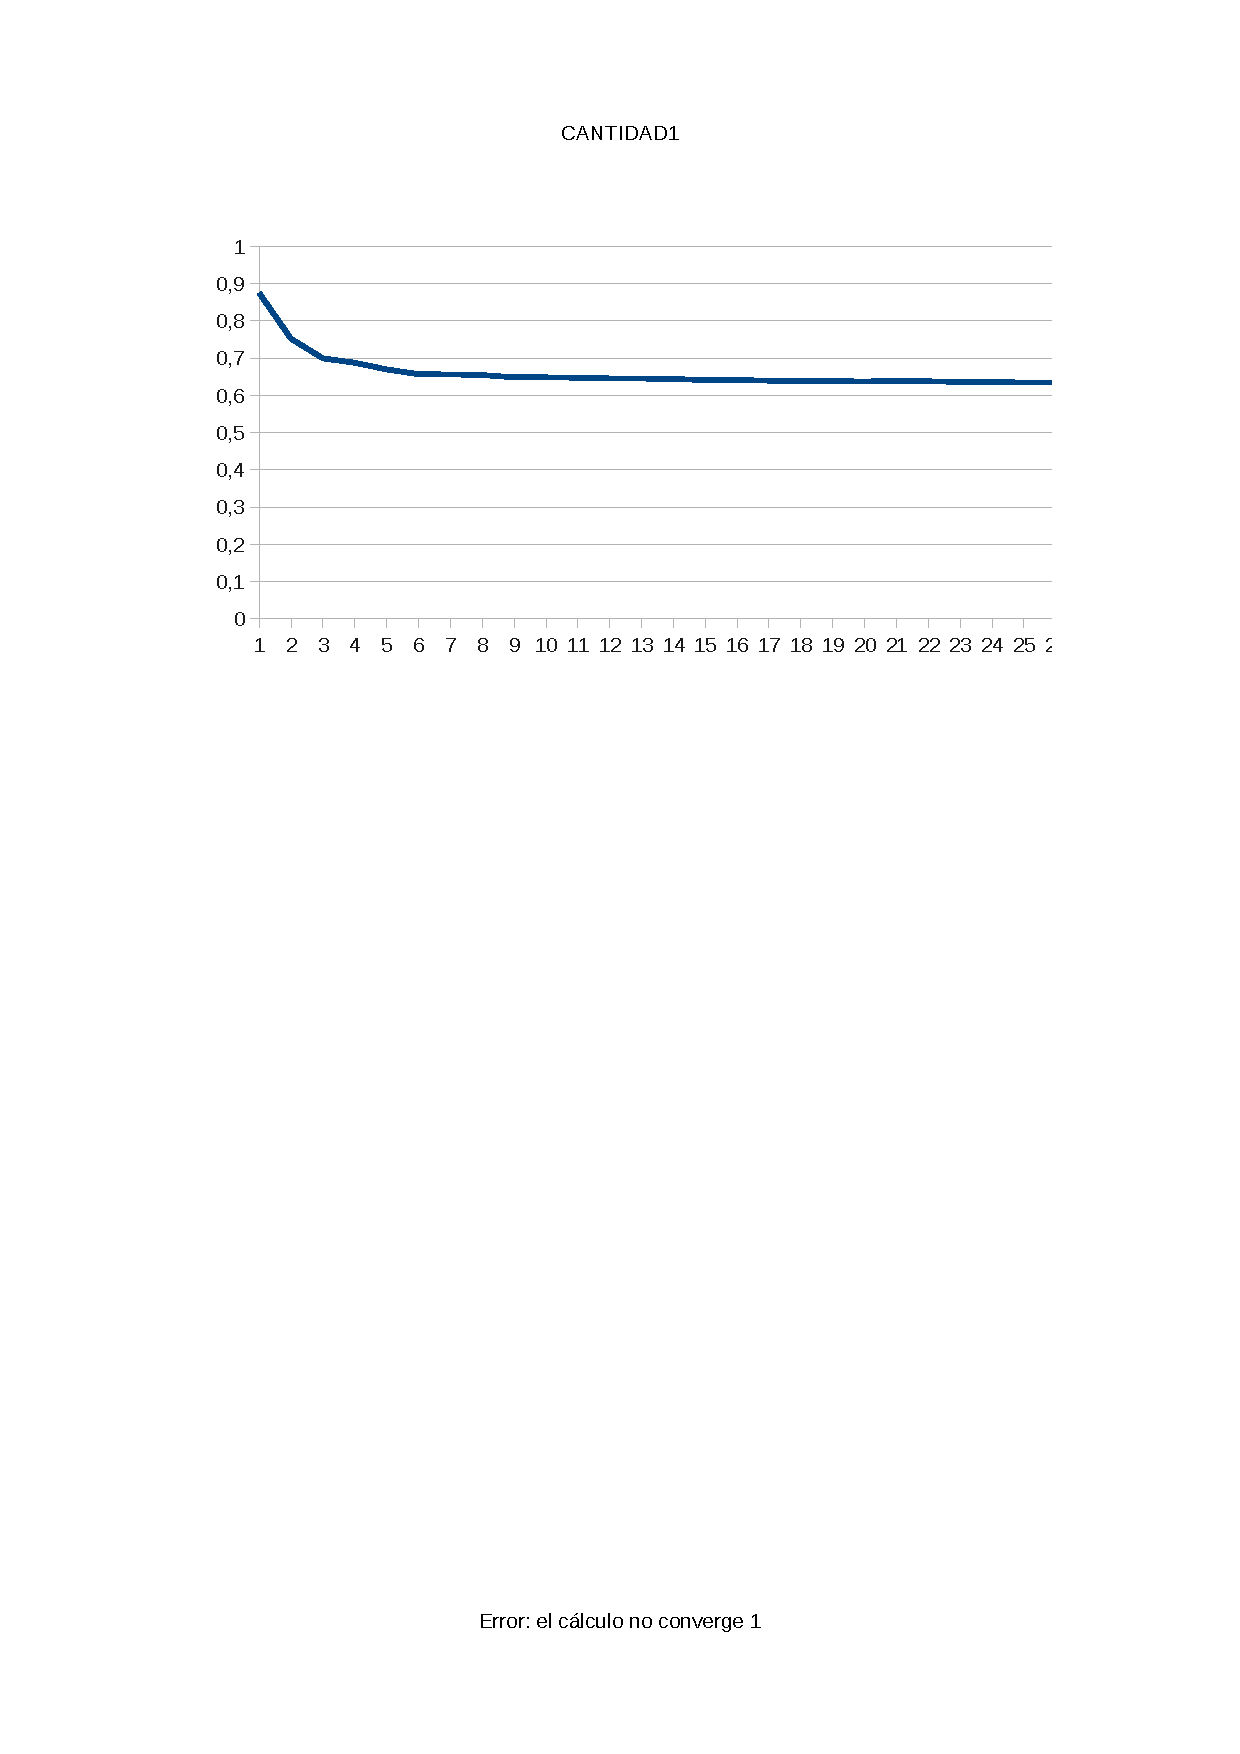
\includegraphics[width=1\textwidth]{img/ic.pdf}
\caption{índice de coincidencia en función de la longitud de clave}
\label{fig:ic}
\end{figure}

\begin{figure}
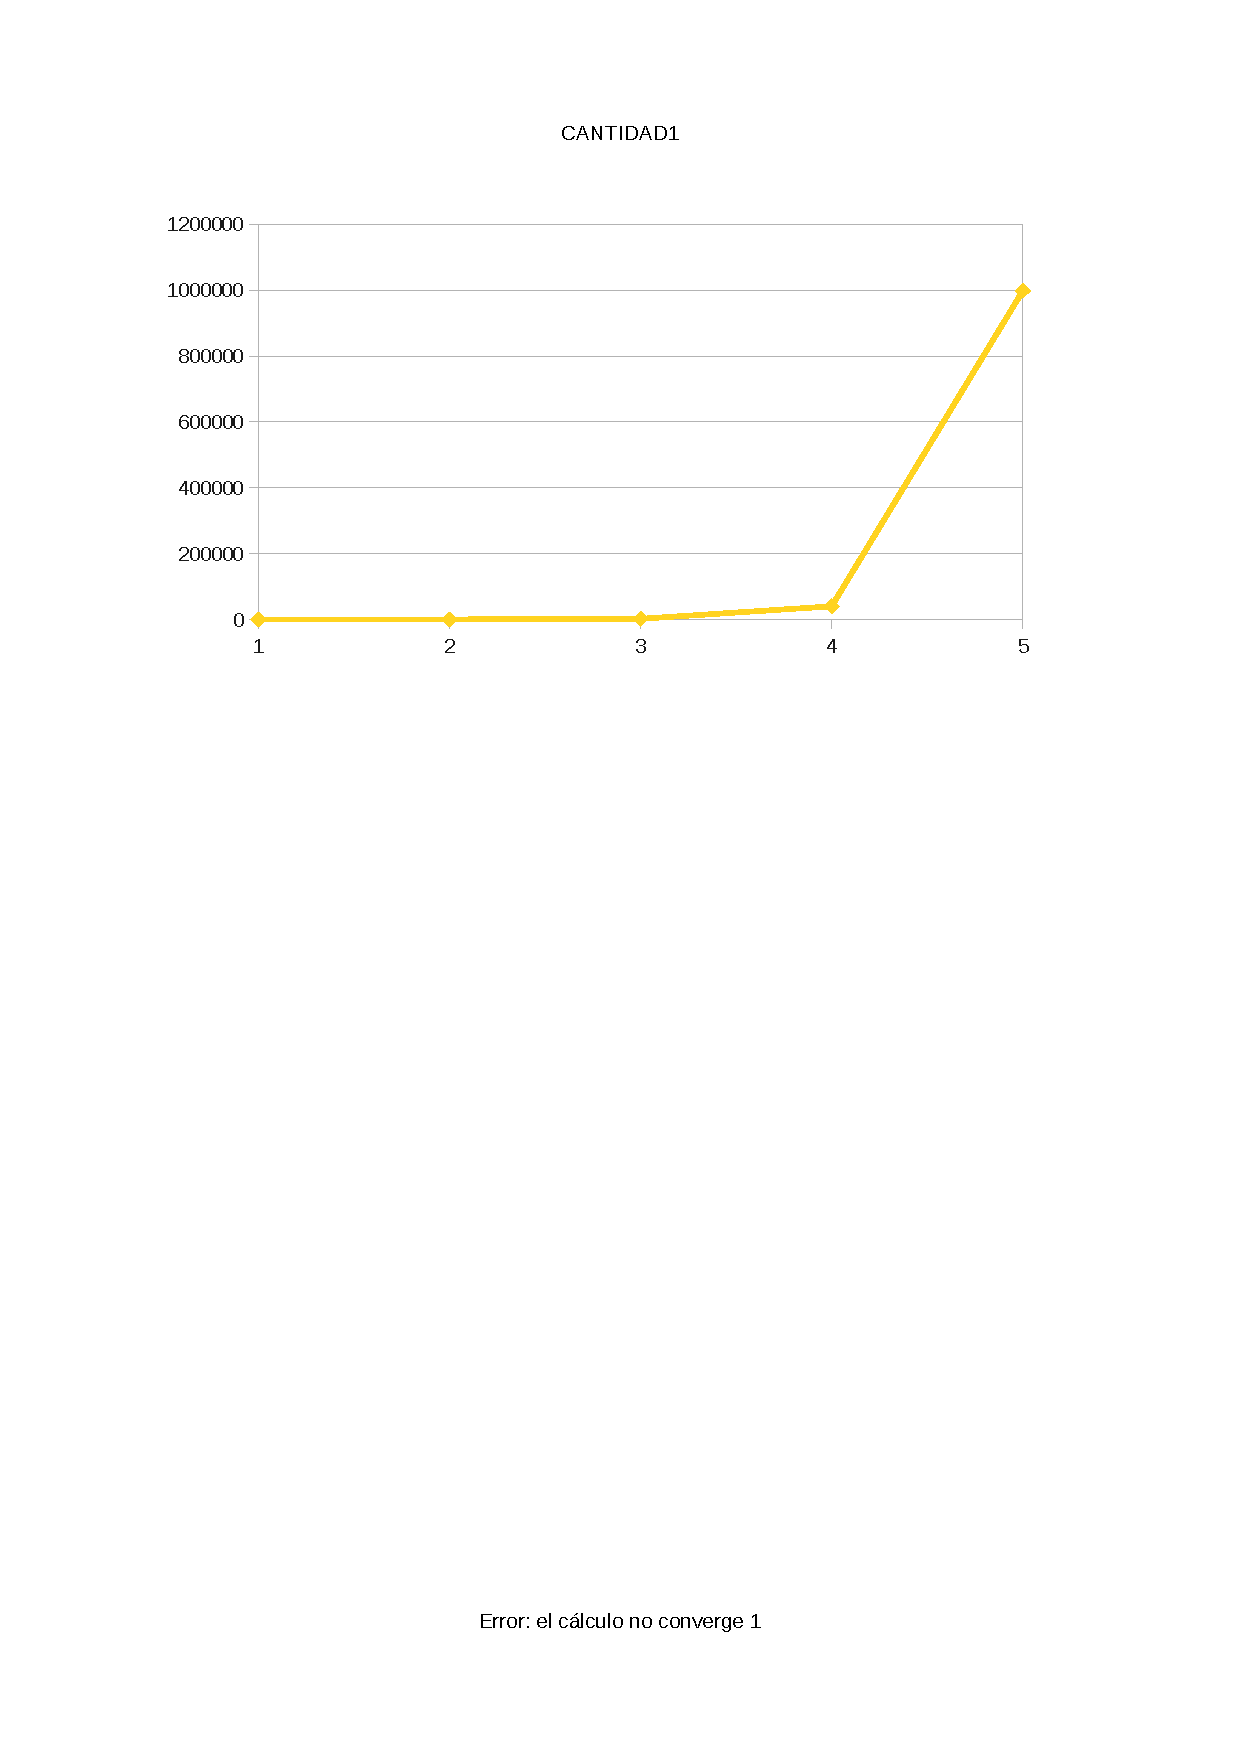
\includegraphics[width=1\textwidth]{img/brute.pdf}
\caption{Fuerza bruta, tiempos en función de la longitud de clave, milisegundos}
\label{fig:brute}
\end{figure}

\begin{figure}
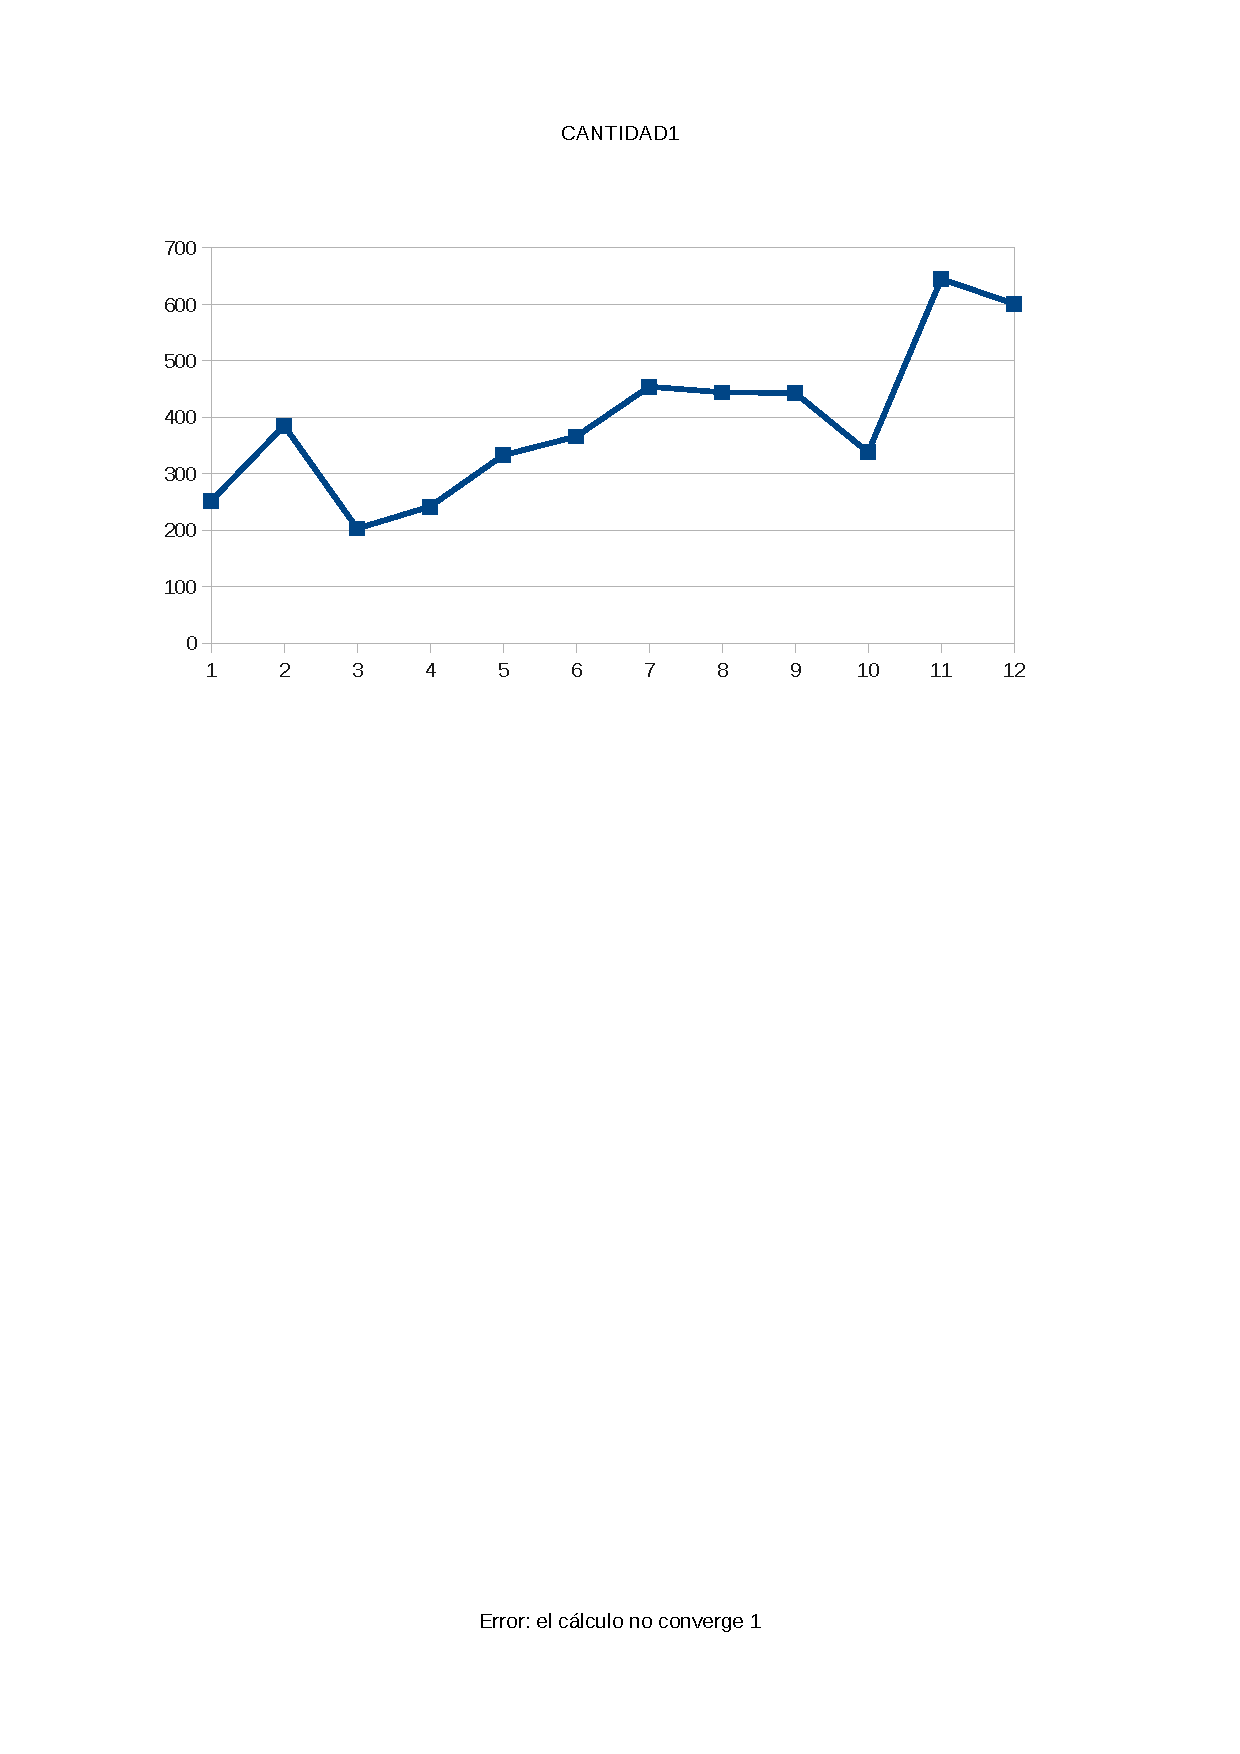
\includegraphics[width=1\textwidth]{img/guess.pdf}
\caption{Algoritmo con tabla de frecuencias, tiempos en función de la longitud de clave, milisegundos}
\label{fig:guess}
\end{figure}

\begin{figure}
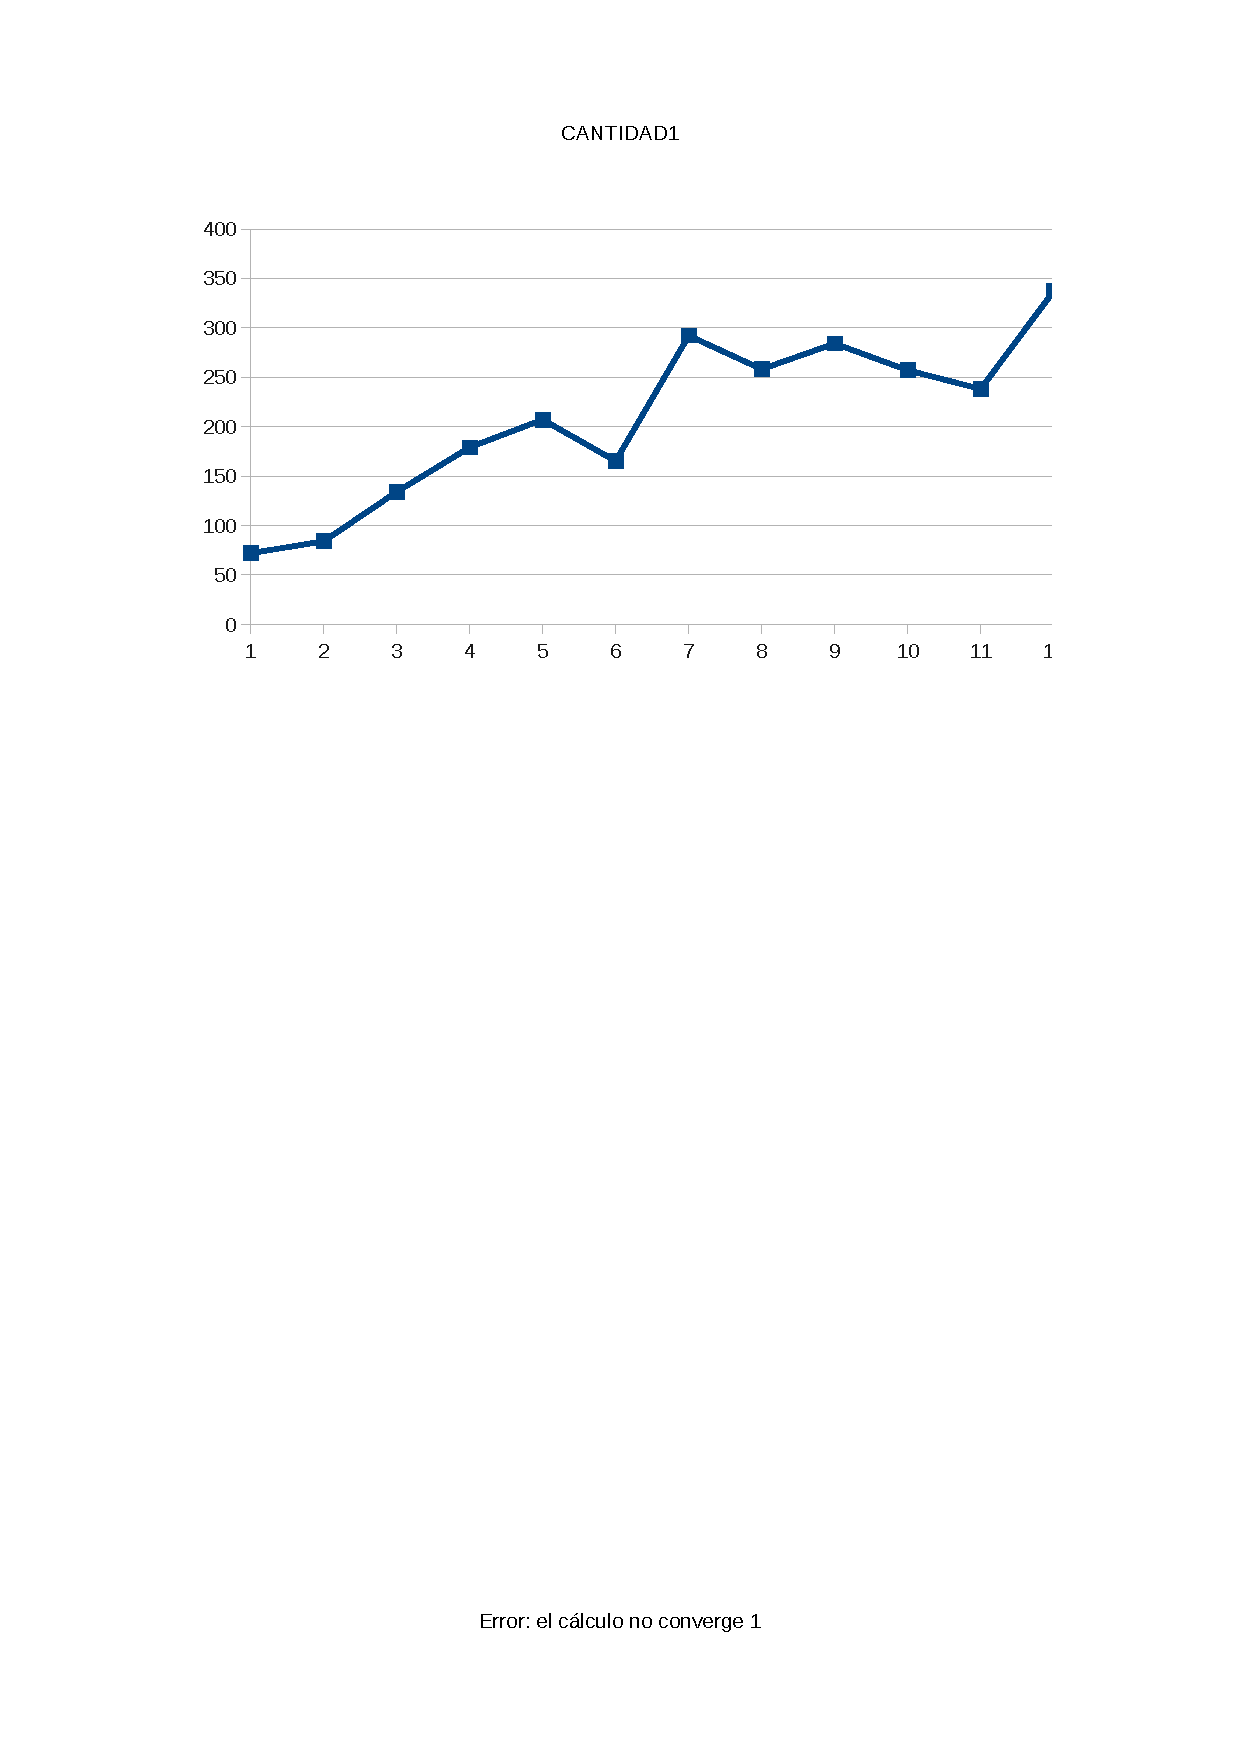
\includegraphics[width=1\textwidth]{img/kg.pdf}
\caption{Tiempos de cálculo de la longitud de clave, milisegundos}
\label{fig:kg}
\end{figure}

\section{Mejoras posibles}
\subsection{Mejora del algoritmo}
Se ha observado que en muchos casos, especialmente cuando se intenta descifrar un texto que emplea una clave larga, el algoritmo
encuentra muchas posibles claves muy similares a la clave correcta. Por ejemplo, si la clave es \texttt{passwordlong}, es probable que
el algoritmo encuentre claves tales como:
\begin{verbatim}
passaordkong
passaordling
\end{verbatim}
Una opción para llegar a la clave real a partir de alguna de las claves parciales, por ejemplo \texttt{passaordkong}, sería realizar un análisis del texto descifrado, buscando palabras mal formadas a las que reemplazándoles caracteres den como resultado una palabra correcta en el idioma. Por ejemplo, podríamos encontrarnos en el texto descifrado palabras como \texttt{housr} y \texttt{orangt}, a las que cambiándoles un carácter, coincidirían con \texttt{house} y \texttt{orange} respectivamente.

En teoría estos caracteres del texto que no corresponden con la palabra original se corresponderían con las partes de la clave que no
son correctas. Calculando el \textit{delta} de los caracteres de estas palabras podríamos corregir partes de la clave y llegar a la clave correcta a partir de una clave similar, en nuestro caso, llegaríamos a \texttt{passwordlong} a partir de \texttt{passaordkong}.

\subsection{Mejora de la implementación}
Como cada una de las pruebas de claves es completamente independiente de las demás, los algoritmos podrían ser fácilmente paralelizados tanto el de fuerza bruta como el de tabla de frecuencias.

\section{Forma de uso}
\texttt{java - jar vigenere-assembly-1.0.jar <parámetros>}

Al menos se le debe indicar uno de los siguientes parámetros
\begin{itemize}
\item -c: Realiza un cifrado
\item -d: Realiza un descrifrado
\item -b: Intenta romper un cifrado usando fuerza bruta
\item -bg: Intenta romper un cifrado adivinando la longitud de la clave
\end{itemize}

Si se elige cifrado o descifrado, se debe especificar con \textit{-k} la clave.

La entrada puede ser un fichero o un argumento por linea de comandos
\begin{itemize}
\item -s: La entrada es el \textit{string} que siga a este argumento
\item -f: La entrada es el fichero proporcionado por este argumento
\end{itemize}

La salida por defecto es la pantalla, con \textit{-o} se puede especificar un fichero de salida.

El alfabeto a utilizar se elige con \textit{-x}, los valores posibles son:
\begin{itemize}
\item A: Mayusculas
\item a: Minusculas
\item 0: Números
\item \$: Símbolos
\end{itemize}

Estos valores para el alfabeto pueden combinarse entre si.


En caso de querer romper un cifrado, se deben proporcionar las siguientes opciones.
\begin{itemize}
\item -l: Longitud máxima posible de la clave
\item -m: Número de palabras encontradas en una solución para que se considere válida. Véase \ref{validate}
\end{itemize}

Otras opciones posibles para romper un cifrado serían
\begin{itemize}
\item -a: Número de caracteres que se prueban cuando se realiza el descifrado por tabla de frecuencia. Por defecto
se prueban todos los caracteres del lenguaje, desde el más probable hasta el menos probable por orden. Véase \ref{partition}
\item -n: Longitud del \textit{snippet} que se descifra para comprobar la validez de la clave, en lugar de descifrar el texto 
completo. Por defecto es 512, un valor que ha funcionado bien en las pruebas. Véase \ref{snippet}
\end{itemize}

\section{Compilación}
Para poder construir el proyecto es necesario tener instalada la herramienta de construcción \textit{sbt}, \url{http://www.scala-sbt.org/}, y \textit{scala} 2.10.4.

Para construir el programa, es necesario ejecutar:
\begin{verbatim}
sbt assembly
\end{verbatim}

Lo cual descargará las dependencias del proyecto, compilará el código fuente y tras pasar los test, generará un \textit{fat jar}, esto es, un fichero \textit{.jar} que contiene todas las dependencias necesarias y puede ser ejecutado directamente con \texttt{java -jar <argumentos del programa>}.
\end{document}

%-------------------------------------------------------------------------------
% SNIPPETS
%-------------------------------------------------------------------------------

%\begin{figure}[!hp]
%   \centering
%   \includegraphics[width=0.8\textwidth]{file_name}
%   \caption{}
%   \centering
%   \label{label:file_name}
%\end{figure}

%\begin{figure}[!hp]
%   \centering
%   \includegraphics[width=0.8\textwidth]{graph}
%   \caption{Blood pressure ranges and associated level of hypertension (American Heart Association, 2013).}
%   \centering
%   \label{label:graph}
%\end{figure}

%\begin{wrapfigure}{r}{0.30\textwidth}
%   \vspace{-40pt}
%   \begin{center}
%       \includegraphics[width=0.29\textwidth]{file_name}
%   \end{center}
%   \vspace{-20pt}
%   \caption{}
%   \label{label:file_name}
%\end{wrapfigure}

%\begin{wrapfigure}{r}{0.45\textwidth}
%   \begin{center}
%       \includegraphics[width=0.29\textwidth]{manometer}
%   \end{center}
%   \caption{Aneroid sphygmomanometer with stethoscope (Medicalexpo, 2012).}
%   \label{label:manometer}
%\end{wrapfigure}

%\begin{table}[!hp]\footnotesize
%   \centering
%   \begin{tabular}{cccccc}
%   \toprule
%   \multicolumn{2}{c} {Pearson's correlation test} & \multicolumn{4}{c} {Independent t-test} \\
%   \midrule    
%   \multicolumn{2}{c} {Gender} & \multicolumn{2}{c} {Activity level} & \multicolumn{2}{c} {Gender} \\
%   \midrule
%   Males & Females & 1st level & 6th level & Males & Females \\
%   \midrule
%   \multicolumn{2}{c} {BMI vs. SP} & \multicolumn{2}{c} {Systolic pressure} & \multicolumn{2}{c} {Systolic Pressure} \\
%   \multicolumn{2}{c} {BMI vs. DP} & \multicolumn{2}{c} {Diastolic pressure} & \multicolumn{2}{c} {Diastolic pressure} \\
%   \multicolumn{2}{c} {BMI vs. MAP} & \multicolumn{2}{c} {MAP} & \multicolumn{2}{c} {MAP} \\
%   \multicolumn{2}{c} {W:H ratio vs. SP} & \multicolumn{2}{c} {BMI} & \multicolumn{2}{c} {BMI} \\
%   \multicolumn{2}{c} {W:H ratio vs. DP} & \multicolumn{2}{c} {W:H ratio} & \multicolumn{2}{c} {W:H ratio} \\
%   \multicolumn{2}{c} {W:H ratio vs. MAP} & \multicolumn{2}{c} {\% Body fat} & \multicolumn{2}{c} {\% Body fat} \\
%   \multicolumn{2}{c} {} & \multicolumn{2}{c} {Height} & \multicolumn{2}{c} {Height} \\
%   \multicolumn{2}{c} {} & \multicolumn{2}{c} {Weight} & \multicolumn{2}{c} {Weight} \\
%   \multicolumn{2}{c} {} & \multicolumn{2}{c} {Heart rate} & \multicolumn{2}{c} {Heart rate} \\
%   \bottomrule
%   \end{tabular}
%   \caption{Parameters that were analysed and related statistical test performed for current study. BMI - body mass index; SP - systolic pressure; DP - diastolic pressure; MAP - mean arterial pressure; W:H ratio - waist to hip ratio.}
%   \label{label:tests}
%\end{table}